\chapter{Introduction}
The increasing proliferation and maturation of electric drive technologies has
caused drive system-level integration to become a high priority in a variety
of application areas including electric propulsion, aerospace, white goods,
and down-hole drilling.
Tight integration of motor and drive electronics
offers attractive properties including reduced overall system volume,
reduction of high-current cabling, reduced radiated EMI, simplified cooling
arrangements, and appealing fault tolerance opportunities.

However, physical integration of electric machines and drives presents many
challenges.
In order to integrate the controls and power electronics into the
machine housing, the power electronics must be designed to operate reliably in
elevated vibration and thermal environments that fall outside of standard
ranges for industrial-grade components.
Further complicating the
challenges, customers for integrated drives typically expect the drive
electronics to meet or exceed the lifetime of the machine, requiring very high
reliability in demanding environments.

Early generations of integrated motor drives have typically used conventional
three-phase induction or PM synchronous machines combined with standard
voltage-source 6-switch bridge inverters to excite the machine.
In many of these units, the drive is housed in its own enclosure which, in
turn, is mounted on the side or end of the machine.
More aggressive concepts for integrated machine drives have been proposed that
approach more closely the ultimate objective of mounting the complete drive
inside the same enclosure as the machine, but commercialization of these
advanced integrated drive architectures has been limited to date.

One of these advanced concepts that has been proposed in the literature is the
integrated modular motor drive (IMMD) .
As illustrated in Fig. \ref{figCPESIMMD}, this
concept segments the stator into individual pole pieces, each encircled by a
concentrated winding that is excited by its own dedicated electronics unit
that includes both the necessary power electronics and controls to form a
complete pole-drive unit.
The IMMD is completed by interconnecting a number
of these pole-drive units to form an annulus around the rotor.
Appealing features of this IMMD concept emerge from its modularity, offering
opportunities for improved manufacturability, enhanced fault tolerance and
redundancy, and simplified repair/replacement of the pole-drive units.

\section{Motivation}

\subsection{Reliability and Redundancy}
As electric drive systems move into many power and actuation applications
previously handled by mechanical and hydraulic systems, reliability and
redundancy becomes an important consideration for an electric drive.

In aerospace systems, a typical fault mitigation method is to use parallel
actuators which are torque summed in order that a failed actuator does not
cause system failure \cite{Annaz09}.
While this method is well understood and robust, it requires significant extra
weight, volume, and cost over a single actuator able to perform the same task.

Argile et al. \cite{Argile08} described a Markov model method for describing
converter faults and calculating the total MTTF for a fault-tolerant converter
model which is able to continue operation even in the face of lost power
conversion components.
This paper shows clearly both the difficulties posed by the increased failure
rates caused by increasing component counts and the opportunities afforded by
fault tolerance when repair is possible.


\subsection{EMI Containment}
As electric drives spread into automotive and residential areas at high
powers, EMI mitigation becomes a major design challenge.



\section{Previous Research}
Previous research into integrated modular motor drives can be split into three
categories.
\subsection{System Level Designs and Integrated Converters}
The first category, system-level research includes investigations into
controlling high phase-order machines and fault tolerant drives to achieve
continued system operation in the presence of machine and drive component
failures.

The first of these investigations was carried out with a load commutated
thyristor based inverter and a 6-phase induction machine.
In his research \cite{Jahns78} T. M. Jahns achieved full torque operation of a faulted
machine with only minimal increase in machine and drive losses though the
modification of applied voltage magnitude and frequency to the remaining
healthy phases.

More recent related research has been undertaken at WEMPEC in the area of
modular converter integration.

Recently Nate Brown and others \cite{Brown07a} have demonstrated a fully
modular machine consisting of tooth-wound SMC pole pieces coupled to a
modularized inverter.
\begin{figure}[htbp]
\centering
\label{figCPESIMMD}
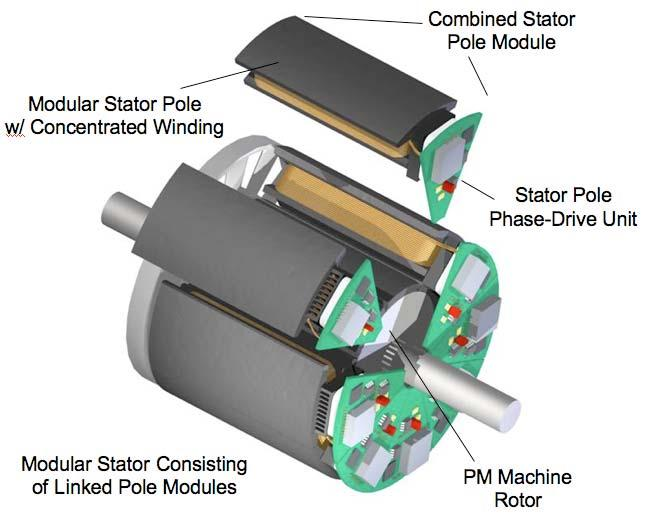
\includegraphics[width=5in]{IMMD3k}
\caption{Rendered views of 5-phase SMC modular motor drive.}
\end{figure}
The entire machine and drive are air cooled by drawing air first through the
inverter poles then through the machine airgap and slots.
The controls on this machine however are still fully centralized.

This modular inverter also demonstrated the difficulties in modular drive
interconnect as its phase and power connections developed intermittent faults
after a relatively short operating life.


\subsection{Machine Design}
The next category and a vital component of any motor control work is the
design of the electric machine itself.

In order to allow easy redundancy and increased flexibility of operating with
multiple phase configurations, this works focuses on a 6-phase machine with a
60 degree phase spacing.
A dual winding 12 slot, 10 pole dual-layer design was chosen due to the
highly isolated and contained flux paths \cite{Bianchi05}.
This design allows for machine characterization and testing using standard 3
phase converters which greatly helps both in model design and system
debugging.


\subsection{Current Sensing}
Accurate current sensing is a vital component of high-performance motor
controls.  Often this is accomplished through the use of transformer-based
hall-effect sensors.  Sadly, for an integrated application these sensors are
both highly temperature sensitive and too large.

A much more compact current sensing method involves the use of free-space
magnetic field sensors in fixed position relative to a current carrying
conductor.
This approach allows both small-size and high bandwidth as current sensor core
materials do not come into play.
In \cite{Schneider10} GMR sensors are used as they allow for extremely large
bandwidth (into the MHz range).
These sensors are however unipolar and biasing magnet requirements offset some
of the thermal stability gains.

